% Section 3: Chapter 1 - Implementation
% Division: 3.1, 3.2, 3.4 (Member A - Pham Tran Anh Quan); 3.3, 3.5 (Member B - Nguyen Tien Cuong).
\section{Chapter 1: Implementation}
\label{sec:03_chapter1_implementation}

% ---------------------------------------------------------------------------
\subsection{The Eclat Algorithm from the Original Paper}
\label{subsec:eclat_algo}
% To be completed by Member A (Zaki 2000 §4.1, §4.2, §5.2; Figure F01).

% ---------------------------------------------------------------------------
\subsection{Complexity Analysis}
\label{subsec:complexity}
% To be completed by Member A.

% ---------------------------------------------------------------------------
\subsection{Software Architecture, SPMF I/O, and Command-Line Interface}
\label{subsec:arch_io}

The system is structured as a standalone Julia package, \texttt{EclatFIM} (Julia~1.11.4), partitioned into three isolated dependency environments: a minimal root package (depending solely on \texttt{DataStructures.jl} and the standard library) for the command-line interface and automated test suite; an experimental environment (\texttt{scripts/}) for benchmarking and figure generation; and an application environment for Chapter~3. Figure~\ref{fig:f02_arch} illustrates the modular architecture and end-to-end data flow of the package.

\begin{figure}[H]
\centering
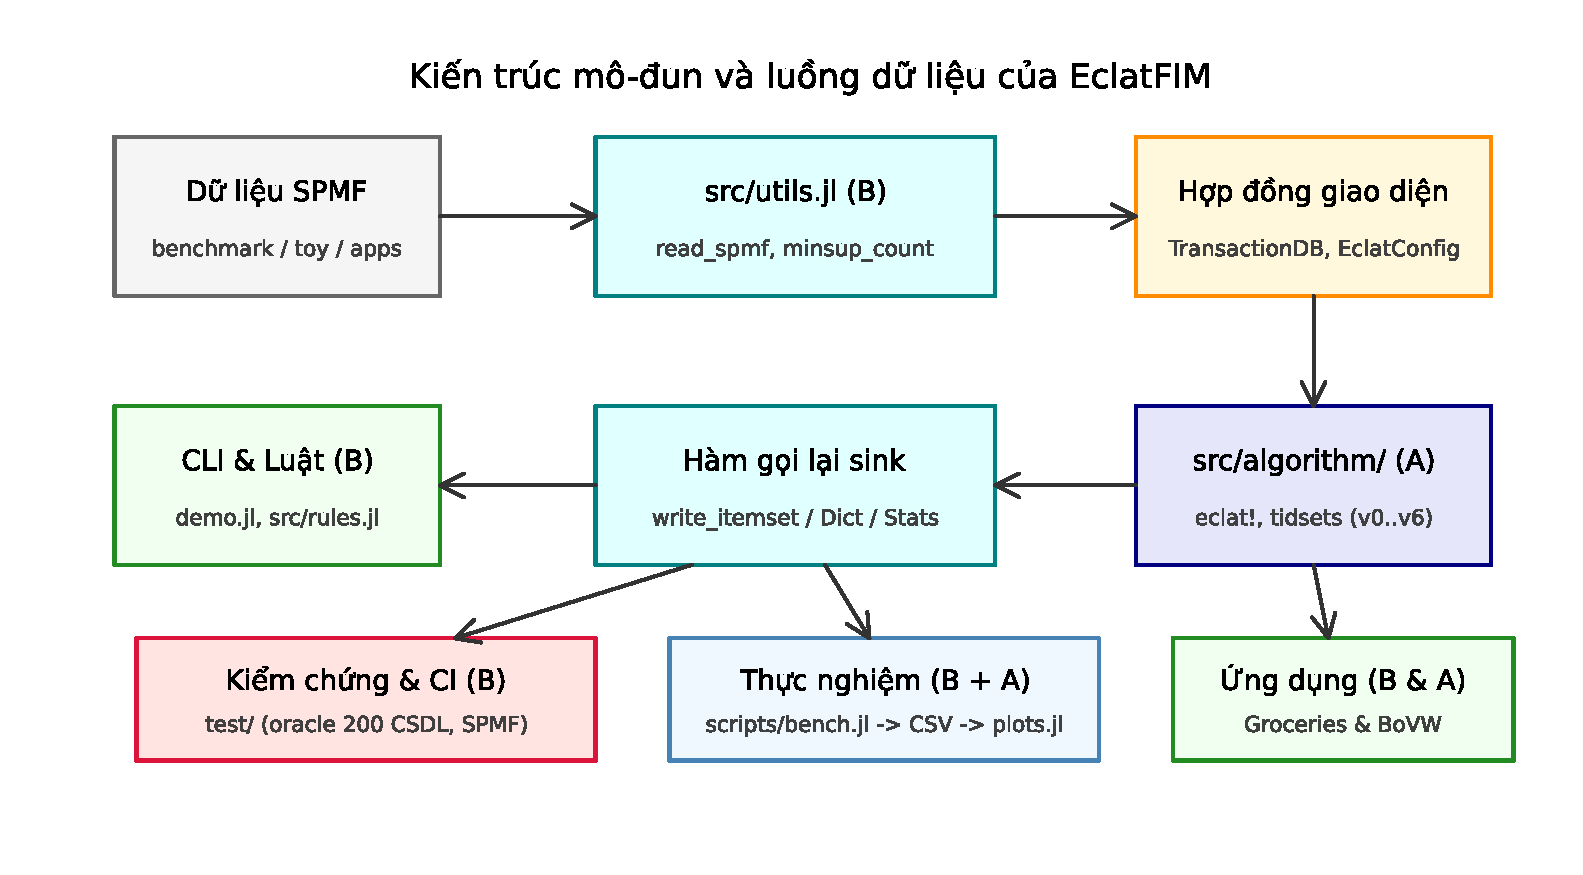
\includegraphics[width=0.92\textwidth]{F02_architecture.pdf}
\caption{Modular architecture and data flow of \texttt{EclatFIM}, separating SPMF-compliant I/O, the interface contract (\texttt{EclatConfig}), the core Eclat mining engine, and downstream verification, benchmarking, and application layers.}
\label{fig:f02_arch}
\end{figure}

The software design centers on three architectural principles:
\begin{enumerate}
    \item \textbf{Decoupled Interface Contract:} The \texttt{TransactionDB} structure maps ascending original item identifiers (\texttt{Int64}) into contiguous internal codes $1 \ldots m$ (\texttt{Int32}), enabling compact array indexing rather than hash-table lookups. The \texttt{EclatConfig} structure decouples independent optimization axes (\texttt{tidset}, \texttt{order}, \texttt{reuse}, \texttt{isect}, \texttt{level2}), allowing a single test suite and benchmarking harness to evaluate every algorithmic variant uniformly without altering call sites.
    \item \textbf{Streaming Output via Callback (\texttt{sink}):} At low minimum support (\texttt{minsup}) thresholds, frequent itemset collections may reach millions of patterns. The core routine \texttt{eclat!(sink, db, minsup, cfg)} emits each frequent itemset through a reusable prefix buffer to \texttt{sink}, allowing direct file streaming without accumulating the entire output set in main memory.
    \item \textbf{Idiomatic Julia Features:} Multiple dispatch specializes tidset intersection operators and eliminates instrumentation overhead at compile time when \texttt{stats === nothing}; generator expressions compute transaction statistics and enumerate proper subsets during rule generation; and \texttt{BinaryMinHeap} and \texttt{counter} from \texttt{DataStructures.jl} extract top-$k$ association rules by lift in $O(n \log k)$ time and tally item frequencies during preprocessing.
\end{enumerate}

To guarantee exact equivalence with the SPMF reference implementation~\cite{fournier2014spmf} (\texttt{spmf.jar}, Eclat v2.65), black-box behavioral experiments were conducted (documented in \texttt{results/spmf\_behavior.md}), establishing two critical I/O conventions:
\begin{itemize}
    \item \emph{Support Threshold Conversion:} SPMF computes the integer support count threshold as $\sigma_{\min} = \lceil \texttt{minsup} \times N \rceil$ using IEEE~754 \texttt{Float64} arithmetic, converting percentage strings \texttt{"p\%"} to $p/100$. Because floating-point rounding can alter boundary outcomes (for example, $0.28 \times 25 = 7.000000000000001$, yielding $\sigma_{\min} = 8$ rather than $7$), \texttt{minsup\_count} reproduces this exact \texttt{Float64} computation to eliminate boundary discrepancies.
    \item \emph{SPMF Parsing and Formatting:} The parser \texttt{read\_spmf} skips empty lines and metadata/comment lines prefixed by \texttt{\#}, \texttt{\%}, or \texttt{@}, and canonicalizes each transaction by sorting and deduplicating items. The writer \texttt{write\_itemset} maps internal codes back to ascending original identifiers, omits the empty itemset, and outputs lines in exact \texttt{i1 i2 ... \#SUP: s} format.
\end{itemize}

The command-line interface \texttt{demo.jl} is implemented without external dependencies and supports \texttt{--minsup} (both ratio and percentage forms), \texttt{-o/--output} (defaulting to \texttt{output.txt}, with \texttt{"-"} streaming patterns to \texttt{stdout} and summary diagnostics to \texttt{stderr}), \texttt{--variant}, and \texttt{--stats}, returning standard exit codes $0$ (success), $1$ (invalid arguments), and $2$ (data or I/O error).

% ---------------------------------------------------------------------------
\subsection{Optimization Techniques}
\label{subsec:optimizations}
% To be completed by Member A (Tables B01, B03, B04 and ablation study v0..v6).

% ---------------------------------------------------------------------------
\subsection{Automated Verification and Match Rate}
\label{subsec:testing}

Correctness is verified independently of the core algorithm author through a three-tier automated testing pipeline located in \texttt{test/}:
\begin{enumerate}
    \item \textbf{Tier 1 — Brute-Force Oracle:} A standalone reference oracle enumerates all $2^m - 1$ non-empty subsets via bitmasks across $200$ randomly generated databases (fixed seeds $1 \ldots 200$, $m \le 12$, $N \le 30$, random $\sigma_{\min}$), verifying $100\%$ exact agreement for every implemented Eclat variant.
    \item \textbf{Tier 2 — Canonical Datasets, Edge Cases, and I/O:} Automated tests validate \texttt{pasquier99.txt} (\texttt{minsup} $= 40\%$, yielding $15$ itemsets) and \texttt{bookstore.txt} from Zaki~\cite{zaki2000scalable} (\texttt{minsup} $= 50\%$, yielding $19$ itemsets, including maximal patterns \texttt{ACTW} and \texttt{CDW}); boundary conditions (empty database, single transaction, identical transactions, \texttt{minsup} $= 100\%$, zero frequent items, large sparse item identifiers); all $10$ floating-point boundary cases of \texttt{minsup\_count}; and hand-verified association rule calculations in \texttt{test\_rules.jl}.
    \item \textbf{Tier 3 — Large-Scale Benchmark Verification:} The comparator \texttt{scripts/compare\_spmf.jl} defines the exact match rate between the implementation's output $\mathcal{F}_{\text{ours}}$ and the SPMF reference output $\mathcal{F}_{\text{SPMF}}$ as:
    \begin{equation}
        \text{Match Rate} = \frac{\left|\{X \in \mathcal{F}_{\text{ours}} \cap \mathcal{F}_{\text{SPMF}} : \sigma_{\text{ours}}(X) = \sigma_{\text{SPMF}}(X)\}\right|}{\left|\mathcal{F}_{\text{ours}} \cup \mathcal{F}_{\text{SPMF}}\right|} \times 100\%.
    \end{equation}
    For outputs exceeding $5 \times 10^6$ itemsets, comparison automatically switches to an order-invariant fingerprint mode: each canonicalized line is hashed with SHA-256, and the leading $64$ bits are accumulated modulo $2^{64}$.
\end{enumerate}

Continuous Integration (GitHub Actions) executes the entire test suite on a clean Julia~1.11.4 environment under both default settings and \texttt{--check-bounds=yes} to verify array-bounds safety for \texttt{@inbounds}-annotated loops. Table~\ref{tab:b02_tests} summarizes the automated verification results across unit tests and four benchmark datasets (\texttt{chess}, \texttt{mushroom}, \texttt{retail}, \texttt{T10I4D100K}).

% Data source: `julia --project=. test/runtests.jl` (commit 52011a2)
\begin{table}[H]
\centering
\caption{Summary of automated test suite execution (\texttt{test/runtests.jl}) for variants \texttt{v0} and \texttt{v1} under default and \texttt{--check-bounds=yes} modes.}
\label{tab:b02_tests}
\begin{tabular}{llrr}
\toprule
Test Group & Source File & Assertions & Pass Rate \\
\midrule
SPMF I/O and \texttt{minsup\_count} & \texttt{test\_io.jl} & 49 & 100\% \\
200-DB brute-force oracle, toy, edge cases & \texttt{test\_correctness.jl} & 62 & 100\% \\
Association rules and \texttt{top\_k} & \texttt{test\_rules.jl} & 225 & 100\% \\
Statistics and cross-variant checks (4 benchmarks) & \texttt{test\_benchmark.jl} & 16 & 100\% \\
\midrule
\textbf{Total} & \texttt{runtests.jl} & \textbf{352} & \textbf{100\%} \\
\bottomrule
\end{tabular}
\end{table}
